\documentclass[12pt]{article}

% sean look for !!! that means it needs work!

\usepackage{amscd} 
\usepackage{amsmath}
\usepackage{amsthm} 
\usepackage{amssymb} 
\usepackage{eufrak}
\usepackage{hyperref}
\usepackage[margin=.85in]{geometry}
\usepackage{float}
\usepackage{graphicx}
\usepackage{caption}
\usepackage{subcaption}
\usepackage{color}

\theoremstyle{plain}
\newtheorem{postulate}{Postulate} 
\newtheorem{theorem}{Theorem}[section]
\newtheorem{corollary}[theorem]{Corollary}
\newtheorem{proposition}[theorem]{Proposition} 
\newtheorem{lemma}[theorem]{Lemma}
\newtheorem{conjecture}[theorem]{Conjecture}
\newtheorem{algorithm}[theorem]{Algorithm}
\theoremstyle{definition} 
\newtheorem{definition}[theorem]{Definition}
\newtheorem{example}[theorem]{Example}

\theoremstyle{remark} 
\newtheorem{remark}[theorem]{Remark} 

\renewcommand{\arraystretch}{1.4}
\newcommand{\Q}{\mathbb{Q}}
\newcommand{\Z}{\mathbb{Z}}
\newcommand{\N}{\mathbb{N}}
\newcommand{\R}{\mathbb{R}}
\newcommand{\C}{\mathbb{C}}
\newcommand{\F}{\mathbb{F}}
\newcommand{\Qhat}{\widehat{Q}^{n}(t)}
\newcommand{\What}{\widehat{W}^{n}(t)}
\newcommand{\Qtild}{\widetilde{Q}^{n}(t)}
\newcommand{\Qfhat}{\widehat{Q}^{n}(\cdot)}
\newcommand{\Wfhat}{\widehat{W}^{n}(\cdot)}
\newcommand{\Qftild}{\widetilde{Q}^{n}(\cdot)}
\newcommand{\error}{E^{n}(\cdot)}

\title{Investigating the Effects of Variance in Markovian Shortest Remaining Processing Time Queues}

\author{
Sean Malter\footnote{Research supported by ViaSat.} \ and Prof.\ Amber L.\ Puha\\
Department of Mathematics, California State University, San Marcos \\
%333 S.\ Twin Oaks Valley Road\\
%San Marcos CA 92096\\
\small{malte002@cougars.csusm.edu \& apuha@csusm.edu}
}


\begin{document}
\maketitle

\begin{abstract}
In this report, we investigate the relationship between the queue length and the workload processes in a
Markovian shortest remaining processing time (SRPT) queue.
We simulate these processes in heavy traffic without drift, i.e. when the arrival and processing rates are equal.
In this setting, the diffusion scaled workload process converges in distribution to a non-degenerate reflected
Brownian motion \cite{igl70}.
However, the diffusion scaled queue length process converges in distribution to the process that is identically equal
to zero \cite{gro11}. We explore how much smaller the order of magnitude is of the rescaled queue length in
comparison to the rescaled workload.
Through simulation we identify a logarithmic correction factor that seems to be valid for any processing rate.
Under this corrective scaling, our simulations suggest that varying the processing rate only effects the limiting variance.
\end{abstract}

\section{Introduction}

Here we investigate the behavior of the queue length process in a Markovian shortest remaining processing time (SRPT) queue via simulation.  Specifically we investigate the effect of variance on the asymptotic behavior of the queue length process in heavy traffic.

\subsection{Shortest Remaining Processing Time Queues}

We model the shortest remaining processing time queue as follows.  We consider a system where jobs arrive one at time according to a Poisson process with rate $0<\lambda<\infty$.  This means that the interarrival times between jobs form a sequence of independent and identically distributed exponential random variables with rate $\lambda$.  Each job has associated with it a processing time, which denotes the amount of time that the job requires from the server.
These processing times are assumed to be drawn from a sequence of positive, independent and identically distributed random
variables that have positive, finite mean $m$ and are independent of the arrival process.  In an SRPT
queue, the job in the system with the shortest remaining processing time is served first, with preemption.
Specifically, when a new job enters the system, it enters service immediately if the system was empty immediately prior to its arrival.
Otherwise, there was a job in service.  In this case, the server determines whether or not the new job has a
smaller processing time than the remaining processing of the job in service.  If the new job has the smaller
of the two processing times, it takes priority and enters service, while the other job is placed on hold. Otherwise, the server continues serving the job in service.
This placing of jobs on hold is known as preemption.  A job exits the system once the server has completely satisfied
its original processing time requirement.  Upon a departure, the server idles if their are no jobs in the system, and begins service of
the job in the system with the shortest remaining processing time otherwise.  We refer to $\rho=\lambda m$ as the utilization.
Such a queue is often denoted by M/G/1/SRPT, where the M refers to the Markovian nature of the arrival process, the
G refers to the general nature of the processing time distribution, 1 refers to the number of servers, and SRPT
refers to the service discipline.  The focus of the work here will actually be on exponentially distributed processing times.  In particular, we focus on the M/M/1/SPRT queue.

SRPT is a naturally interesting service discipline to study.  Indeed, it is performance optimal with respect to queue length since it is the queue length minimizer over all nonidling service disciplines \cite{sch68, smi76}.  Here nonidling refers to service disciplines in which the server doesn't idling unless the system is empty.  However, there is  an anticipated performance trade off.  For this, we refer to the total length of time that that a job spends in the system as its sojourn or response time.  It is anticipated that jobs with large processing times will experience lengthy sojourn times. This trade off has been explored in \cite{dow09}, where it is demonstrated that the growth rate of the sojourn times is determined by the decay rate of the tail of the processing time distribution.  The focus here is on quantifying the queue length minimization property of SRPT.

\subsection{Background on Heavy Traffic Diffusion Limits}
Our investigation involves exploiting the established behavior of the so called workload process $(W(t),t\ge 0)$ in
heavy traffic.  The value $W(t)$ of the workload at time $t$ is the total amount of time that the server would need to work in order to completely serve all jobs in the system at time $t$, ignoring future arrivals.  A classic result in \cite{igl70} establishes that under standard heavy traffic assumptions the diffusion scaled workload process converges in distribution to a non-degenerate reflected Brownian motion $(W^*(t),t\ge 0)$.  Heavy traffic refers to a sequence of systems $\{(W^n(t),t\ge 0)\}_{n\in\N}$ indexed by the natural numbers ${\mathbb N}$ that satisfy certain asymptotic conditions, including the utilization $\rho^n$ approaching one at rate $1/\sqrt{n}$.  Specifically,  for some $\beta\in\R$,
$$
\lim_{n\to\infty} \sqrt{n}\left( 1- \rho^n\right) =\beta.
$$
Diffusion scaling, also known as functional central limit theorem scaling, occurs when time in the $n$th system is scaled by a factor of $n$ and space is scaled by a factor of $1/\sqrt{n}$.  In particular, for $n\in{\mathbb N}$,
\begin{equation}\label{eq:What}
\What=\frac{W^n(nt)}{\sqrt{n}},\qquad t\in[0,\infty).
\end{equation}
The result in \cite{igl70} specifies conditions under which $\Wfhat$ convergence in distribution to $W^*(\cdot)$
as $n$ tends to infinity, where $W^*(\cdot)$ is reflected Brownian motion with drift $\beta$ and positive variance determined by the limiting variances of the interarrival and processing times.
The result in \cite{igl70} generalizes the well-known Donsker's theorem, which specifies conditions under which a centered diffusion
scaled random walk converges in distribution to Brownian motion \cite[Theorem 6.6]{dur95}.  We further note that the
result in \cite{igl70} holds for all nonidling service disciplines. In particular, it holds for SRPT.

Recently \cite{gro11} investigated the behavior of the SRPT queue length process $\left(Q(t),t\ge 0\right)$
in heavy traffic.  Here $Q(t)$ is the number of jobs in the system at time $t$.  They showed that, if the service time distribution has unbounded support, then the diffusion scaled queue length process $\left(\widehat{Q}^n(t), t\ge 0\right)$ converges in distribution to the process that is identically equal to zero under standard heavy traffic conditions.
This is in contrast to what happens for other natural nonidling service disciplines such as first-come first-serve (FCFS) or processor sharing (PS).  In these cases, the queue length process converges in distribution to a nondegenerate diffusion limit $(Q^*(t),t\ge 0)$ that is a positive constant multiple of $\left(W^*(t),t\ge 0\right)$.  In particular, for FCFS, $Q^*(t)= W^*(t)/m$ for $t\ge 0$, where $m$ is the mean of the limiting processing time distribution \cite{igl70}.  While for PS, $Q^*(t)= W^*(t)/m^*$ for $t\ge 0$, where $m^*$ is positive and uniquely determined by the limiting processing time distribution \cite{gro04}.  But it seems that the queue length minimizing nature of SRPT forces the constant to be zero for the SRPT discipline. In particular, the order of magnitude of the queue length process is actually smaller than the workload process. This in and of itself is quite interesting.
The natural next question to ask is whether or not one can determine the correct order of magnitude for the queue length process.

\subsection{Suspected Behavior of the Queue Length Process}
The earlier work \cite{dow09} on fluid limits for SRPT queues potentially developed some insight regarding the order of magnitude of the queue length process.
We describe this in the special case where the utilization converges to one, arrival rate converges to $\lambda$, the
fluid scaled initial queue length converges in distribution to a positive constant $q_0$, the distribution of the initial processing
times converges to a continuous distribution with probability density function $g$, and the distribution of the processing times for jobs that
arrive after time zero converges to a continuous distribution with strictly positive probability density function $f$.  Then define
$$
s(x)=\frac{ q_0\int_0^x y g(y) dy }{\lambda\int_x^{\infty} y f(y) dy},\qquad\hbox{for }x\in[0,\infty).
$$
The value $s(x)$ turns out to represent the departure time of jobs in the system at time zero that have initial processing
time $x$, in what is known as a fluid limit.  Fluid limits are first order, determinist (functional law of large numbers) approximations.  So one might refer to $s(\cdot)$ as a fluid analog of the sojourn or response time.
In this case, $s(\cdot)$ is continuous,
strictly increasing, and maps onto $[0,\infty)$.  Therefore $s(\cdot)$ has well defined inverse $s^{-1}(t)$ for all $t\ge 0$.
This inverse turns out to be the fluid limit of the frontier process $(F(t),t\ge 0)$, where $F(t)$ denotes the largest
processing of time of any job that has entered service by time $t$ \cite[Theorem 5.20]{dow09}.  Because of this relationship, Puha wondered if $s^{-1}(\cdot)$
could provide the corrective scaling for the queue length process under diffusion scaling.  In particular, Puha wished to investigate
the possibility that
\begin{equation}\label{eq:main}
\widehat W^n(t) \approx s^{-1}(\sqrt{n}) \widehat Q^n(t),\qquad\hbox{for } t\in[0,\infty)\hbox{ as }n\to\infty.
\end{equation}
Here multiplication by $s^{-1}(\sqrt{n})$ has the effect of modifying the spatial scaling.

That \eqref{eq:main} is a reasonable idea to investigate is supported by recent work in \cite{lin11}.
These authors study the expected response time in steady state.  Recall that a response time is associated with each job in the system.
For a given job, it is the total amount of time that the job is in the system, counted from the moment of arrival to the moment of departure.  The expected response time $E[T]$ in steady state is a performance measure that is of importance to the customer.  But the manager is interested in the utilization $\rho$.  In \cite{lin11},
the authors determine the rate at which $E[T]$ grows as a function of the utilization. Interestingly, the growth
rate identified by \cite{lin11} is the same as that predicted by \eqref{eq:main}.  Little's law \cite{sti91} predicts that under reasonable conditions,
the expected response time and queue length are of the same order of magnitude. In particular, Little's law states that mean queue length $E[Q]$ in steady state should satisfy $E[Q] = \lambda E[T]$. And so, if Little's law holds for SRPT, \eqref{eq:main} should follow.

\subsection{Prior Investigation}

Last summer in work supported by ViaSat, Hunsperger and Puha \cite{puhahan12} investigated whether or not \eqref{eq:main} holds via simulation.  They pursued this by considering two classes of processing time distributions, the Weibull and Pareto distributions.  The complementary Pareto distribution function decays polynomially, while the complementary Weibull distribution function decays faster than polynomially.  Hence, these two classes provide a range of distinct behaviors to test against.  Further,  exact computations are relatively easy for these two classes.  For this work, they set $\lambda=1$.  Then in order to enforce the heavy traffic condition, the parameters of the processing time distribution were chosen such that $m=1$.
They found that \eqref{eq:main} seems to be valid for one specific instance of the Weibull distribution, the exponential case with $\lambda=1$.  Recall that the probability density function for a rate $\lambda$ exponential random variable is given by
$$
f(x)=\lambda \exp(-\lambda x),\qquad x\ge 0.
$$
In the case $\lambda=1$, \eqref{eq:main} suggests adding a factor of $\ln(\sqrt{n})$ to the spatial scaling.  So rather than multiplication by $1/\sqrt{n}$ one multiplies by $\ln(\sqrt{n})/\sqrt{n}$.  They also found that the scaling in \eqref{eq:main} may not be correct for the nonexponential case.  This is rather interesting as it suggests that Little's law may not hold for SRPT.  They indicate that further investigation is required to formulate a new guess as to how workload and queue length are related in heavy traffic.

\subsection{Overview of the Present Investigation}
The work here is a follow on to the work of Hunsperger and Puha \cite{puhahan12}.  We focus on the case of exponential service times, i.e., the M/M/1/SPRT queue.  However, we explore the effect of variance by allowing the arrival rate $\lambda$ to vary.  In particular, we consider an M/M/1/SRPT queue with arrival rate $\lambda>0$ and mean processing time $m>0$ satisfying
$\lambda m=1$.  Then, for $n\in\N$, let
\begin{equation}\label{eq:Qtild}
 \Qtild=\ln\left(\sqrt{n}\right)\widehat Q^n(t)=\frac{\ln(\sqrt{n})Q(nt)}{\sqrt{n}},\qquad t\in[0,\infty).
\end{equation}
The Hunsperger and Puha \cite{puhahan12} simulations suggest that for $\lambda=1$,
under standard heavy traffic assumptions, $\Qftild$ converges in distribution to $W^*(\cdot)$
as $n$ tends to infinity.  One anticipates that the correction factor
$\ln(\sqrt{n})$ applies for all $\lambda>0$.  Here we explore the validity of this expectation.  Our investigation starts with the premise that for some positive constant $C$ that does not depend on $n$, but may depend on $\lambda$,
\begin{equation}\label{eq:C}
C\Wfhat \approx \Qftild, \qquad\hbox{as }n\to\infty.
\end{equation}
More precisely, we anticipate that under suitable heavy traffic conditions there exists a positive constant $C$ such that
$\Qftild$ converges in distribution to $CW^*(\cdot)$ as $n$ tends to infinity.

We test the viability of this convergence via simulation and find extensive evidence in support.  These simulations suggest that $C=\lambda$.  This is summarized in Section \ref{sec:ratio}.  In Section \ref{sec:scaling}, the appropriately rescaled workload and queue length processes are plotted on a common plots for various values of $\lambda$ and large values of $n$ to demonstrate that the two processes are becoming close.  In Section \ref{sec:error}, we plot the difference between the two processes to make it more apparent that they aren't very far apart.  Finally, in Section \ref{sec:tables}, we compute the maximum absolute difference of the rescaled workload and queue length processes for series of values of $n$ over the time interval $[0,1]$ for different values of $\lambda$.  We  demonstrate that for each given value of $\lambda$, the maximum error seems to be decreasing as $n$ increases.  This is meant to provide evidence in favor of the following statement:  for all $T,\varepsilon, \eta>0$, 
\begin{equation} \label{eq:proof}
\liminf_{n\to\infty} P\left( \sup_{t\in[0,T]}\left| C\What - \Qtild \right| \le \varepsilon\right)\ge 1-\eta. 
\end{equation}
Ultimately, we would like to develop a mathematical proof of the above relationship, which could be used to prove
the asserted convergence in distribution.  In the remainder of this report, we explain our methodology and present the simulation results that led to our conclusions.

% Section About R and modeling SRPT
\section{Implementing R to Simulate SRPT Queues}

We simulate the queue length and workload processes in an M/M/1/SRPT queue with the aid of the programming language R.  We had many suitable choices for these simulations.  However, the language R has many built in
functions that aided in creating graphics and statistical computing.   Creating these simulations required us to
determine what information to track and store.  We chose to focus on the times $t$ at which a job arrived to or
departed from the queue. In particular, our code keeps track of a 3-tuple that includes the update time and the
queue length and workload at that time.
Our code has two input parameters, the scaling index $n$ and the arrival rate $\lambda$.  Then,
in order to satisfy the heavy traffic condition, we set the mean processing time $m$ to be the reciprocal of
$\lambda$.  In particular, $\lambda^n=\lambda$ and $m^n=1/\lambda$, so that $\rho^n=\lambda^nm^n=1$ throughout.  Therefore, it follows that we are simulating the case where the limiting arrival rate is $\lambda$ and the drift $\beta$ is 0.
Then, the heavy traffic diffusion limit $W^*(\cdot)$ of the workload process is a reflected Brownian motion with zero drift. 
Further, the variance of $W^*(\cdot)$ is given by $2/\lambda$.
Since $W^*(\cdot)$ has variance
$2/\lambda$,
the limiting variance varies with $\lambda$.  Hence, by using difference values of $\lambda$ and $n$, we were
able to explore the effect of variance on the rescaled queue length and workload processes as $n$ increases.



% section about finding C
\section{Identifying the Constant $C$}\label{sec:ratio}

If a $C$ satisfying \eqref{eq:C} exists, then the ratio

\begin{equation}\label{eq:ratio}
\frac{\Wfhat}{\Qftild}
\end{equation}
must approach a flat line as $n$ becomes large.  In particular, it must
be the case that, as $n$ becomes large,
\begin{equation}\label{eq:R}
\frac{\Wfhat}{\Qftild} \approx \frac{1}{C}.
\end{equation}
To investigate this, we plotted \eqref{eq:ratio} for different values of $\lambda$, fairly large values of $n$, and $t\in[0,1/\lambda]$.  In such plots we expect to see a relatively flat graph, with a bit of randomness, but the height of the approximately flat line may vary with $\lambda$.  These ratio plots are problematic for times $t$ such that $Q(nt) = 0$.  Note that if $Q(nt) = 0$ at time $t$, then there are no jobs in the system at time $t$ and
so $W(nt) = 0$ at time $t$.  But we can't a priori assume what value to substitute for the ratio at this specific time.
To address this issue, we use the convention that we do not plot a value at time points $t$ for which $Q(nt) = 0$.  In other words, those time points are simply skipped.

%talk about how we plot it
As we began our computations of \eqref{eq:ratio}, we were interested in creating plots over the time interval $[0,1]$ with a large fixed $n$ for various values of $\lambda$. We had good results with $n=10^{7}$ for $\lambda = 1$ and $\lambda = 0.2$. But, when $\lambda = 5$ our computers could not handle the larger data sets created in this case.
We needed a method to handle the larger $\lambda$ cases, while also staying consistent with our choice for $n$. We found that plotting over time intervals $[0,1/\lambda]$ would best fit our criteria to generate data sets of similar size.  This is because the expected number of arrivals in $[0,1/\lambda]$ is $\lambda n^7/\lambda = n^7$. Therefore the number of iterations required in our code was of order $n^7$ for any $\lambda$.

% lambda = 1 ratio plot
\begin{figure}[H]
\centering
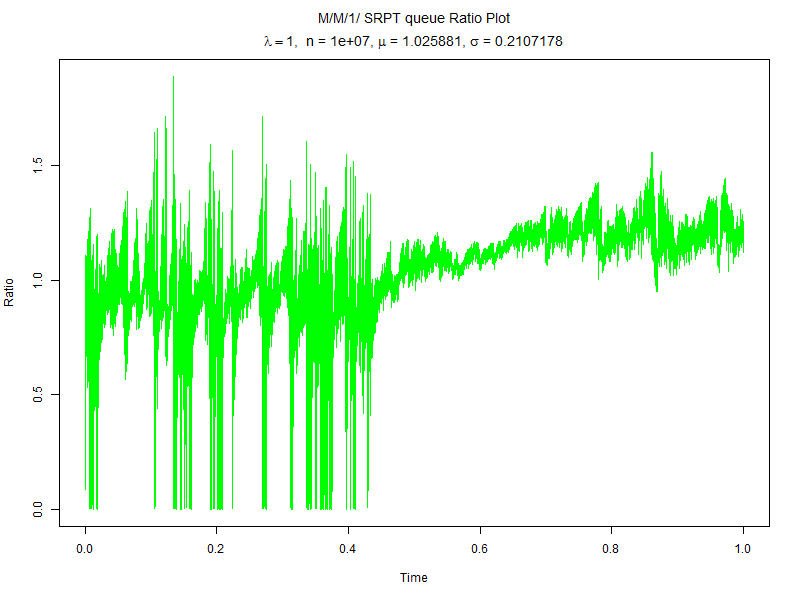
\includegraphics[width = 460px]{Pictures/ratio1.png}
\caption{This is a plot of \eqref{eq:ratio} with $\lambda = 1$ and $n = 10^{7}$. Here we denote $\mu$ as the average value and $\sigma$ the standard deviation of \eqref{eq:ratio} over $[0,1]$. We see in this plot the average is slightly above one. This figure met our expectation that the ratio should be relatively flat with some randomness. We see that larger fluctuations of the ratio occur for smaller values of $t$. As $t$ approaches 1, the plot levels off with small excursions around the horizontal line $y = 1/\lambda = 1$.}
\label{fig:ratio1}
\end{figure}

%make a note of the time scaling

%side by side ratio graphs
\begin{figure}[H]
\centering
\begin{subfigure}[t]{9cm}
\centering
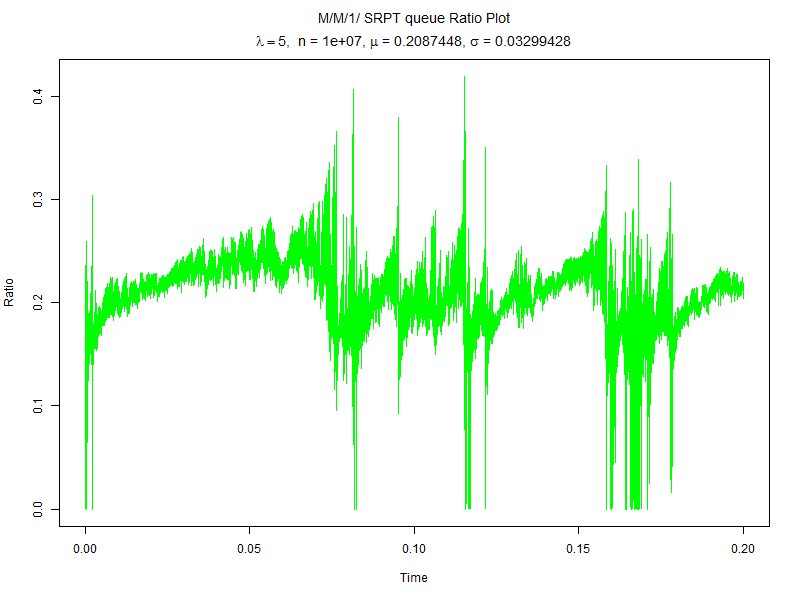
\includegraphics[width=9cm]{Pictures/ratio5.png}
\label{fig:ratio5}
\captionsetup{width = 8cm}
\caption{This is a plot of \eqref{eq:ratio} with $\lambda = 5$ and $n = 10^{7}$. Again we have $\mu$ denoting the average value and $\sigma$ denotes the standard deviation of \eqref{eq:ratio} over $[0,1/\lambda]$. Note how close the average $\mu = 0.2087$ is to $1/\lambda = 0.2$. This figure is a good example of random movement around the line $y = 1/\lambda = 1/5$, with some clusters of larger fluctuations. The movement in this plot seemed to be typical for plots with larger values of $\lambda$, possibly due to the smaller variances of interarrival and processing times.}
\end{subfigure}%
\begin{subfigure}[t]{9cm}
\centering
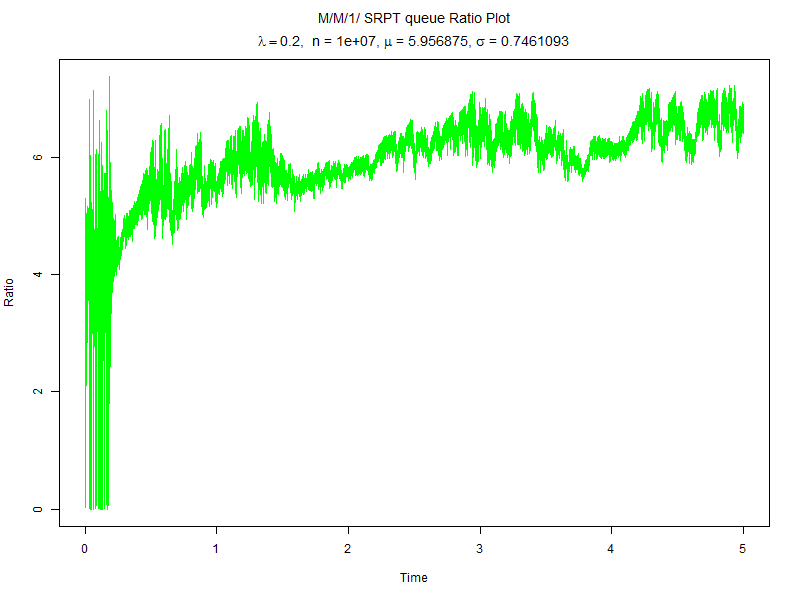
\includegraphics[width=9cm]{Pictures/ratio02.png}
\label{fig:ratio02}
\captionsetup{width=8cm}
\caption{In this plot of \eqref{eq:ratio}, we have $\lambda = 0.2$ and $n = 10^{7}$. We see in this figure the average $\mu = 5.957$ is much larger than what we expected $(1/\lambda = 5)$. For smaller values of $\lambda$, we generally saw longer excursions of \eqref{eq:ratio} above our guessed horizontal line $y = 1/\lambda$, which resulted in the average $\mu$ being larger than what we expected.}
\end{subfigure}
\end{figure}

These figures provide evidence that there exists a $C$ satisfying \eqref{eq:R}. Each plot seems to be approaching that of a horizontal line.  There are brief excursions below the line, that correspond to times where the system empties.   There are also longer, but less amplified excursions, above the horizontal line, possibly due to some large jobs being introduced to the queue or due to the nature of SRPT minimizing queue length. These figures provided empirical evidence that the reciprocal of the average $\mu$ of \eqref{eq:ratio} over $t \in [0, 1/\lambda]$ might be a good estimator of $C$.  The average $\mu$ is typically very close to $1/\lambda$, leading us to the speculate that $C = \lambda$ satisfies \eqref{eq:R}.  Naturally we wanted to investigate how the average of \eqref{eq:ratio} behaves for many values of $\lambda$, and whether or not our projected value for $C$ seems to hold for these different values
of $\lambda$.  Table \ref{tab:ratio} corresponds to \eqref{eq:ratio} for $n = 10^{6}$ over $t \in [0, 1/\lambda]$.  In the table, we record the statistic $1/\mu$ to make it easier to see that $1/\mu \approx \lambda$.  This table seems to support that $C=\lambda$ satisfies \eqref{eq:R}.

%table of ratio
\begin{table}[H]
\caption{\label{tab:ratio}}
\vspace{-0.5cm}
\begin{center}
\begin{tabular}{| c | l | l |}
\hline
\multicolumn{3}{ | c | } {Table for \eqref{eq:ratio}, with $n = 10^{6}$ and $t \in [0,1/\lambda]$}\\
\hline \hline
$\lambda$ & \multicolumn{1}{| c |}{$1/\mu$} & \multicolumn{1}{| c |}{$\sigma$}  \\
\hline
0.1 & 0.105471448028813 & 2.58401055272361\\
0.5 & 0.504537711481153 & 0.36280620384928\\
0.7 & 0.657587748417663 & 0.248152077644996\\
1 & 0.869920091652271 & 0.155238462713735\\
2 & 1.97216348457889 & 0.0916511133213832\\
5 & 5.02771079857985 & 0.0412554733286094\\
13 & 13.0244084241662 & 0.0139554623512711\\
\hline
\end{tabular}
\end{center}
\end{table}

As we see from Table \ref{tab:ratio}, the statistic $1/\mu \approx \lambda$ in most cases. We see the largest difference between $\lambda$ and $1/\mu$ when $\lambda = 1$, with $\lambda - 1/\mu \approx 0.13$. Generally the results of this table were as expected, finding a strong relation between the average of the plots of \eqref{eq:ratio} and the choice of $\lambda$. As we varied $\lambda$, we found that the inverse $1/\mu$ of the average was closely related to the choice of $\lambda$.

% puha's graph and words
\begin{minipage}[t]{6cm}
\begin{figure}[H]
\centering
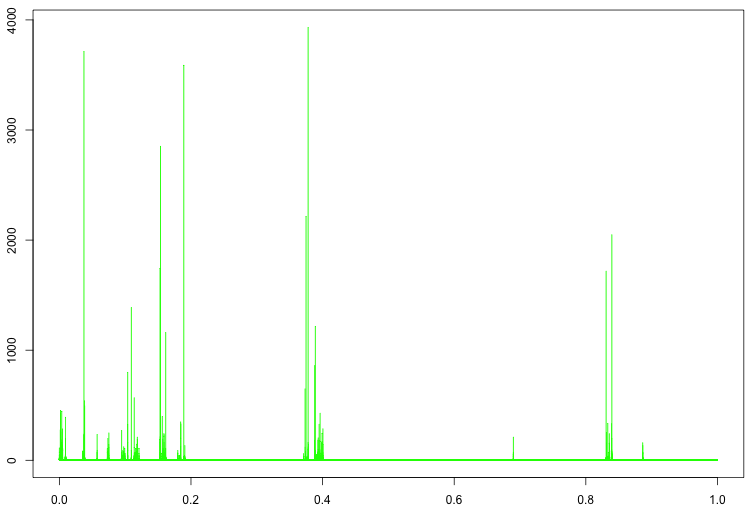
\includegraphics[width=6cm]{Pictures/altRatio.png}
\label{fig:altRatio}
\end{figure}
\end{minipage}
\qquad
\begin{minipage}[t]{10cm}
\vspace*{\baselineskip}
As a side note, we also tried to plot the reciprocal of the ratio in \eqref{eq:ratio}.  Those plots also tended to look relatively constant (flat).  However there were brief, huge spikes.  This suggested that workload tends to zero faster than queue length at times as those.  In this regard, note $\Qftild$ is a discrete valued object, so is bounded away from zero when it is not zero.  Hence, plotting the ratio in \eqref{eq:ratio} more effectively illustrated the results.
\end{minipage}
\vspace*{\baselineskip}

Recall that the variance of the reflected Brownian motion limit $W^*(\cdot)$ in the case of an M/M/1/SRPT queue
with limiting arrival rate $\lambda$ is given by $2/\lambda$.  Hence, it follows that
$\lambda W^{*}(\cdot)$ has variance $2\lambda$.  In particular, we speculate that under suitable heavy traffic conditions
$\Qftild$ converges in distribution to a reflected Brownian motion $Q^*(\cdot)$ with variance $2\lambda$.
Note that multiplication of $W^*(\cdot)$ by $\lambda$ is equivalent to division by the mean processing time
so that on average each job contributes the mean processing time to the queue length.
This same phenomenon occurs for the M/M/1 FCFS queue, but under standard diffusion scaling.

% Wt vs Qt plots and stuff
\section{Results of Nonstandard Spacial Scaling} \label{sec:scaling}

In this section, We introduce our choice of $C$, namely $C = \lambda$. Throughout we refer to \eqref{eq:Qtild} as the rescaled queue length process and $C\Wfhat$ as the rescaled workload process. In the following figures we plot the rescaled workload and queue length processes on a common graph with a large $n$ and various values of $\lambda$. These graphics are meant to illustrate the relationship between the two processes and the relative closeness of them. 

In the simulating these processes, our choices for $n$ and the length of the time interval were limited due to computational limitations. As we varied $\lambda$, we chose $n = 10^{7}$ and $t \in [0, 1/\lambda]$. The scaling of time in this manner kept the number of points in each plot relatively consistent as we varied $\lambda$. This convention was introduced in Section \ref{sec:ratio} and is used here again for computability when generating plots for different $\lambda$ values. Figures \ref{fig:normalPlot1}, \ref{fig:normalPlot5}, and \ref {fig:normalPlot02} contain plots of the simulations of the two rescaled processes for various values of $\lambda$.


% lambda = 1 norm plot
\begin{figure}[H]
\begin{subfigure}{9cm}
\centering
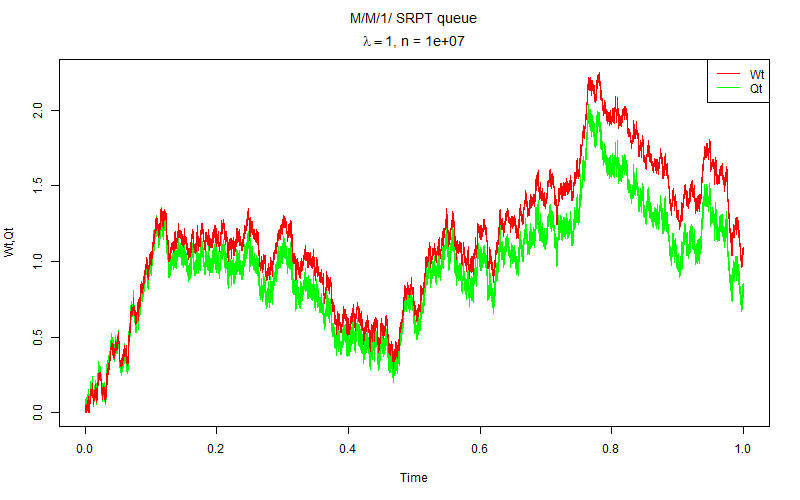
\includegraphics[width = 9cm]{Pictures/normalPlot1_2.png}
\end{subfigure}%
\begin{subfigure}{9cm}
\centering
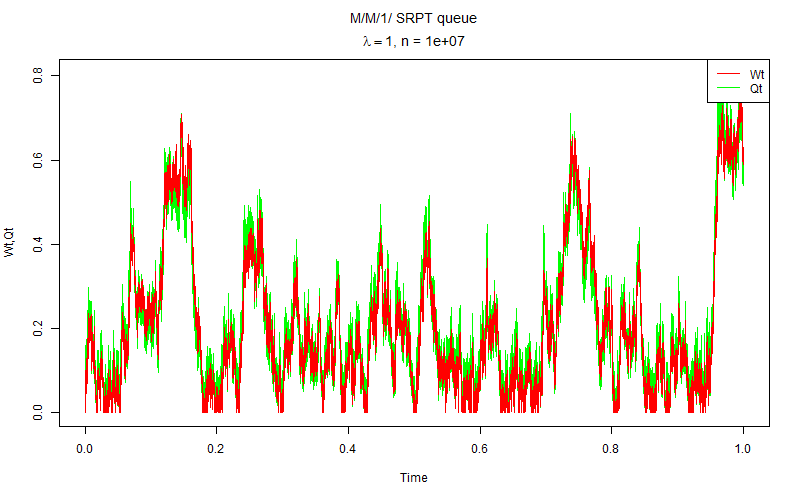
\includegraphics[width = 9cm]{Pictures/normalPlot1_1.png}
\end{subfigure}
\caption{In these two plots, we have $\lambda = 1$ and $n = 10^{7}$ with $t \in [0,1/\lambda]$. The figure on the left is a very typical outcome of the plot with $\lambda = 1$. In both plots we see relatively small separation of the workload and queue length. These plots suggest that $C=\lambda$ is the appropriate multiplicative factor for the workload in the case where $\lambda = 1$.}
\label{fig:normalPlot1}
\end{figure}

The results from our $\lambda = 1$ plots were expected from the previous simulations of Hunsperger and Puha \cite{puhahan12}. We can graphically see the relatively small errors, providing additional support that $\ln ( \sqrt{n})$ is the appropriate correction factor applied to $\Qfhat$ and $C = \lambda$ is the appropriate multiplicative factor for $\Wfhat$ in the case where $\lambda = 1$. Next, we introduce our new results with the scaling $C = \lambda$ for new values of $\lambda$.

% lambda = 5 norm plot
\begin{figure}[H]
\centering
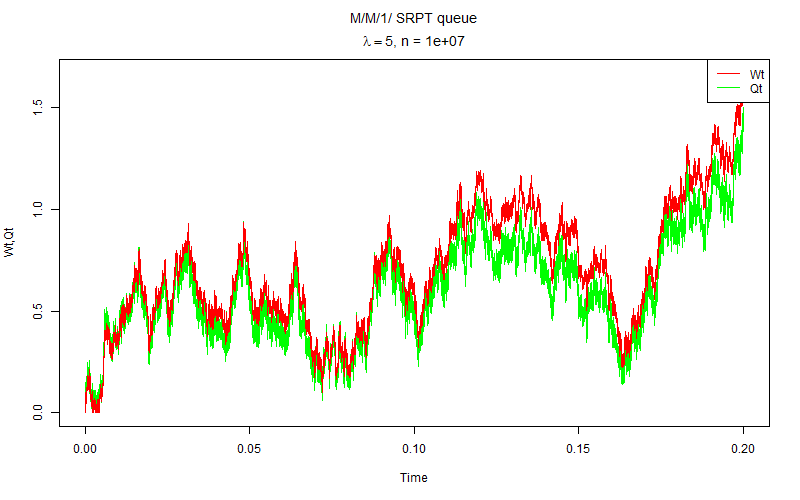
\includegraphics[width = \textwidth]{Pictures/normalPlot5.png}
\caption{In this figure we have $\lambda = 5$ and $n = 10^{7}$ with $t \in [0,1/5]$. Note how close the workload and queue length are in this plot, the closeness of the two processes was typical in our simulation with larger values of $\lambda$. We see the largest separation in the tail end of this plot, with the rescaled workload rising above the rescaled queue length. In our simulations at the time of largest separation, we consistently saw the rescaled workload rising a bit above the rescaled queue length.}
\label{fig:normalPlot5}
\end{figure}

% lambda = 0.2 norm plot
\begin{figure}[H]
\centering
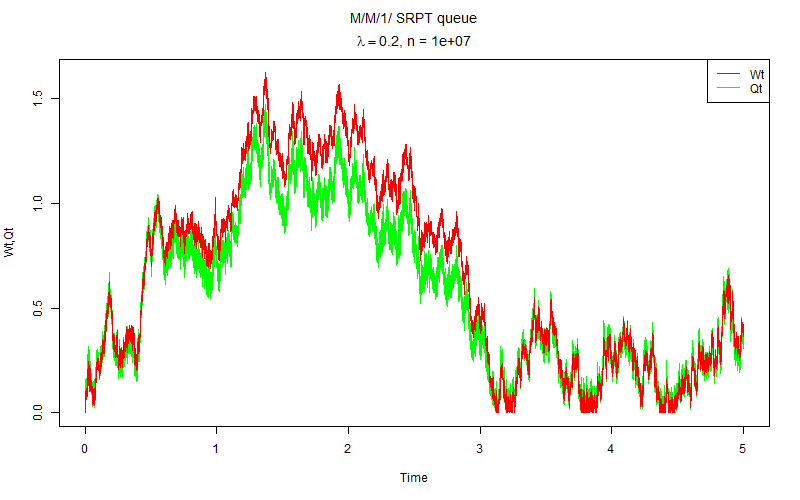
\includegraphics[width = \textwidth]{Pictures/normalPlot02.png}
\caption{In this figure we have $\lambda = 0.2$ and $n=10^{7}$ with $t \in [0, 1/\lambda]$. Note how close the two processes are in this plot, and again we see the workload rising above the queue length for a brief period of time.}
\label{fig:normalPlot02}
\end{figure}

The results of our simulations provided reasonable evidence supporting \eqref{eq:C} with $C=\lambda$. After creating these simulations we became interested in what the difference of the two processes looks like graphically. In otherwords, we ask the question how far apart are the two processes. In the following section we use our simulations associated with the plots in Figures \ref{fig:normalPlot5} and \ref{fig:normalPlot02} to create a new plots to better understand the relationship between the rescaled workload and queue length processes in an SRPT queue.

\section{Further Developing the Relation Between Processes} \label{sec:error}
We further explore the relationship between the two processes by creating a plot of the difference between the rescaled workload and queue length processes. For this, we define the error $E^{n}(\cdot)$ as
\begin{equation} \label{eq:error}
E^{n}(\cdot) = \lambda \Wfhat - \Qftild.
\end{equation}
In Figure \ref{fig:errorPlot5} we present a plot of \eqref{eq:error} for the sample paths in Figure \ref{fig:normalPlot5}. We were also interested in how much of this error could be caused by a single large job. Therefore we include the largest residual service time rescaled by $1/\sqrt{n}$, which is plotted in red. We will denote this as $R[Qt]$ for convenience. So $R[Qt]$ is the rescaled remaining processing time of the job in the system needing the most processing time.


% lambda = 5 error plot
\begin{figure}[H]
\centering
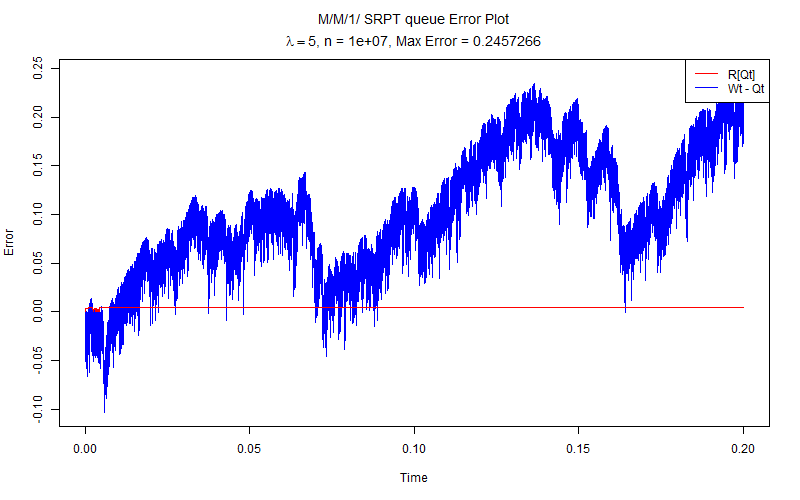
\includegraphics[width = \textwidth]{Pictures/errorPlot5.png}
\caption{We use the data in Figure \ref{fig:normalPlot5} to generate the error as defined in \eqref{eq:error} and the rescaled largest residual service time $R[Qt]$, displayed in blue and red respectively. We see that the error in this figure is generally positive, with the largest error of 0.2457266 at the tail end of the plot. Note the general shape of \eqref{eq:error}, with larger excursions above the y-axis. This movement of the error was typical for our simulations. We also see that the $R[Qt]$ is roughly constant for most of the plot. Perhaps there was a job introduced at $t \approx 0.01$ with a large process time that stayed in queue throughout. It does not appear that this one job accounts for the entire error or even a positive fraction of the error.}
\label{fig:errorPlot5}
\end{figure}


% lambda = 0.2 error plot
\begin{figure}[H]
\centering
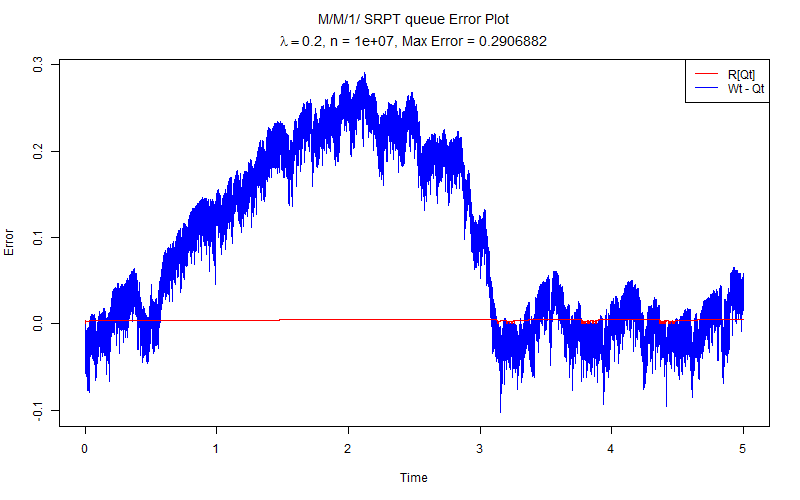
\includegraphics[width = \textwidth]{Pictures/errorPlot02.png}
\caption{This figure is the error of the two processes and the rescaled largest residual service times from Figure \ref{fig:normalPlot02}. We again see the largest excursion above the y-axis. Note that the maximum error presented in this plot is fairly similar to the maximum error in Figure \ref{fig:errorPlot5}. We also see a similar shape of the errors. One of the main difference in the two figures is the length of the excursion in this plot is much longer than those of Figure \ref{fig:errorPlot5}. Another is that the maximum error occours well before the tail end of the plot.}
\label{fig:errorPlot02}
\end{figure}

The results of these plots reflect the tendency of the rescaled workload to be larger than the rescaled queue length in our simulations. As we reflected on our correction factor of $\ln ( \sqrt{n})/\sqrt{n}$ to the queue length and $1/\sqrt{n}$ to the workload, we realize that as n grows the rescaled queue length doesn't shrink as much as the rescaled workload. Hence, this tendency seemed reasonable to us. We were interested in investigating if this error would tend to shrink as $n$ grows larger. We wanted to introduce a larger $n$, for example $n = 10^8$. However, these plots would have ten times more data points in each plot with the current time scaling. Our machines couldn't handle the raw data produced from the plots with $n=10^8$ and $t \in [0,1/\lambda]$. So we created new code that could handle these larger values of $n$. This is introduced it in Section \ref{sec:tables}.


\section{Simulations for Larger $n$} \label{sec:tables}

The above figures provided a good general idea of the shape and movement of the two rescaled processes.
Our next area of interest was to apply larger values of $n$ to our simulations to see if the correction factors applied to the two rescaled processes would minimize their differences.
In our early attempts we encountered some problems creating these simulations.
As mentioned in the end of Section \ref{sec:error}, with our current code, we were unable to create plots of the two processes with $n=10^8$, $\lambda = 1$ and $t \in [0,1/\lambda]$.
We needed a new method to run simulations for larger $n$.
Since we had a good idea of the tendencies of the two rescaled processes, we decided that plotting these processes was no longer necessary. We instead created code that only returns the maximum error of these processes over our time interval.
We defined the maximum error $M$ of the two processes as
\begin{equation} \label{eq:maxerror}
M = \max_{t\in[0,1]} \left | \lambda \What - \Qtild \right |.
\end{equation}
The advantage here is that this can be calculated as a running maximum. Hence, there is no longer a need to store massive queue length and workload process vectors.

Although with this new code we were less limited in our choice of $n$ and our time interval due to storage and retrieval, we were still limited by how much runtime we were willing to dedicate to complete a single sample.
Below we present several tables that summarize our results for the maximum error. In each of the tables, $\lambda$ is fixed. The sample size denotes the number of sample paths generated for the given values of $n$. In particular, for $\lambda = 1$ and $n=10^5$, we generated 100 sample paths over our time interval $[0,1]$.
Then $M$ denotes the maximum error for each path as defined in \eqref{eq:maxerror}.
Hence $M$ is a random variable, of which we generated 100 independent samples. In our tables, $\mu$ is the average value of $M$ over our samples and $\sigma$ is the sample standard deviation. Then $P(M \leq x)$ denotes the probability that $M$ is less than or equal to $x$. We estimate this by counting the number of samples less than or equal to $x$ and dividing by the associated sample size.

% table lambda = 1
\begin{table}[h]
\begin{center}
\begin{minipage}[t]{8.2cm}
\caption{} \label{tab:maxError02}
\begin{tabular}[t]{ | l | c | c | c | c |}
\hline
\multicolumn{5}{| c |}{$\lambda = 0.2$ Unbiased Estimators}\\
\hline \hline
\multicolumn{1}{| c |}{Sample Size} & 100 & 100 & 100 & 25\\ \hline
\multicolumn{1}{| c |}{$n$} & $10^{5}$ & $10^{6}$ & $10^{7}$ & $10^{8}$\\ \hline
\multicolumn{1}{| c |}{$\mu$} & 0.211 & 0.149 & 0.107 & 0.086\\ \hline
\multicolumn{1}{| c |}{$\sigma$} & 0.031 & 0.023 & 0.020 & 0.026\\ \hline
$P(M\leq.05)$	&0	&0	&0	&0\\
$P(M\leq.1)$	&0	&0	&0.39	&0.8\\
$P(M\leq.15)$&0	&0.57	&0.96	&0.96\\
$P(M\leq.2)$ & 0.43 	&0.97	&1	&1\\
\hline
\end{tabular}
\end{minipage}
\quad
\begin{minipage}[t]{8.2cm}
\caption{} \label{tab:maxError06}
\begin{tabular}[t]{ | l | c | c | c | c |}
\hline
\multicolumn{5}{| c |}{$\lambda = 0.6$ Unbiased Estimators}\\
\hline \hline
\multicolumn{1}{| c |}{Sample Size} & 100 & 100 & 100 & 25\\ \hline
\multicolumn{1}{| c |}{$n$} & $10^{5}$ & $10^{6}$ & $10^{7}$ & $10^{8}$\\ \hline
\multicolumn{1}{| c |}{$\mu$} & 0.270& 0.226& 0.210& 0.209\\ \hline
\multicolumn{1}{| c |}{$\sigma$} & 	0.071& 0.085& 0.099& 0.098\\ \hline
$P(M \leq 0.05)$&	0&	0&	0&	0\\
$P(M \leq 0.1)$&	0&	0&	0.04&	0.2\\
$P(M \leq 0.15)$&	0&	0.2&	0.41&	0.32\\
$P(M \leq 0.2)$&	0.06&	0.47&	0.58&	0.44\\
$P(M \leq 0.25)$&	0.49&	0.69&	0.66&	0.72\\
$P(M \leq 0.3)$&	0.8&	0.85&	0.81&	0.84\\
$P(M \leq 0.35)$&	0.87&	0.9&	0.88&	0.92\\
$P(M \leq 0.4)$&	0.94&	0.93&	0.96&	0.96\\
$P(M \leq 0.45)$&	0.96&	0.98&	1&	1\\
$P(M \leq 0.5)$&	0.98&	1&	1&	1\\
\hline
\end{tabular}
\end{minipage}
\end{center}
\end{table}

\begin{table}[H]
\begin{center}
\caption{} \label{tab:maxError1}
\begin{tabular}[t]{ | l | c | c | c | c |}
\hline
\multicolumn{5}{| c |}{$\lambda = 1$ Unbiased Estimators}\\
\hline \hline
\multicolumn{1}{| c |}{Sample Size} & 100 & 100 & 100 & 25\\ \hline
\multicolumn{1}{| c |}{$n$} & $10^{5}$ & $10^{6}$ & $10^{7}$ & $10^{8}$\\ \hline
\multicolumn{1}{| c |}{$\mu$} & 0.347 & 0.309 & 0.301 & 0.270\\ \hline
\multicolumn{1}{| c |}{$\sigma$} &	0.143 & 0.140 & 0.150 & 0.129\\ \hline
$P(M \leq 0.1)$ & 0 & 0 & 0.01 & 0.04\\
$P(M \leq 0.15)$ & 0 & 0.03 & 0.17 & 0.16\\
$P(M \leq 0.2)$	& 0 & 0.31 & 0.31 & 0.4\\
$P(M \leq 0.25)$ & 0.28 & 0.41	 & 0.46 & 0.56\\
$P(M \leq 0.3)$	& 0.52 & 0.54 & 0.56 & 0.64\\
$P(M \leq 0.35)$ & 0.63 & 0.69 & 0.67 & 0.76\\
$P(M \leq 0.4)$	& 0.77 & 0.76 & 0.73 & 0.84\\
$P(M \leq 0.45)$ & 0.83 & 0.84 & 0.79 & 0.88\\
$P(M \leq 0.5)$	& 0.88 & 0.88 & 0.85 & 0.96\\
\hline
\end{tabular}
\end{center}
\end{table}

For $n=10^8$, each $\lambda=1$ sample took about 5 hours of computing time to generate.  So the 25 samples used to generate the summary statistics in the table took about 125 hours, or about 5.2 days to generate.  Therefore, it was impractical to attempt to generate more than 25 samples.  For symmetry, we only generated 25 samples for $\lambda=0.2$ and $n=10^8$, even though these only took about an hour each to generate.  Since the maximum error seems to be converging to zero more rapidly for $\lambda=0.2$, generating these samples seemed less important than getting samples for larger values of $\lambda$.
Tables \ref{tab:maxError3} and \ref{tab:maxError5} provide statistical evidence related to the maximum error $M$ of our simulations for larger values of $\lambda$.

\begin{table}[H]
\begin{center}
\begin{minipage}[t]{8cm}
\caption{} \label{tab:maxError3}
\begin{tabular}[t]{ | l | c | c | c | c |}
\hline
\multicolumn{5}{| c |}{$\lambda = 3$ Unbiased Estimators}\\
\hline \hline
\multicolumn{1}{| c |}{Sample Size} & 100 & 100 & 100 & 25\\ \hline
\multicolumn{1}{| c |}{$n$} & $10^{5}$ & $10^{6}$ & $10^{7}$ & $10^{8}$\\ \hline
\multicolumn{1}{| c |}{$\mu$} & 0.718 & 0.681 & 0.632 & 0.560\\ \hline
\multicolumn{1}{| c |}{$\sigma$} & 	0.387&	0.324&	0.298&	0.365\\ \hline
$P(M \leq 0.1)$&	0.00&	0.00&	0.00&	0.00\\
$P(M \leq 0.2)$&	0.00&	0.01&	0.03&	0.00\\
$P(M \leq 0.3)$&	0.07&	0.09&	0.09&	0.16\\
$P(M \leq 0.4)$&	0.23&	0.20&	0.20&	0.36\\
$P(M \leq 0.5)$&	0.37&	0.38&	0.45&	0.64\\
$P(M \leq 0.6)$&	0.49&	0.46&	0.53&	0.72\\
$P(M \leq 0.7)$&	0.59&	0.55&	0.62&	0.84\\
$P(M \leq 0.8)$&	0.65&	0.68&	0.72&	0.84\\
$P(M \leq 0.9)$&	0.72&	0.75&	0.80&	0.92\\
$P(M \leq 1)$ &	0.76&	0.80&	0.88&	0.92\\
$P(M \leq 1.1)$&	0.84&	0.89&	0.93&	0.92\\
$P(M \leq 1.2)$&	0.88&	0.93&	0.95&	0.92\\
\hline
\end{tabular}
\end{minipage}
\qquad
\begin{minipage}[t]{6.5cm}
\caption{} \label{tab:maxError5}
\begin{tabular}[t]{| l | c | c | c|}
\hline
\multicolumn{4}{| c |}{$\lambda = 5$ Unbiased Estimators}\\
\hline \hline
\multicolumn{1}{| c |}{Sample Size} & 100 & 100 & 100 \\ \hline
\multicolumn{1}{| c |}{$n$} & $10^{5}$ & $10^{6}$ & $10^{7}$\\ \hline
\multicolumn{1}{| c |}{$\mu$} & 1.091 & 0.935 & 0.870\\ \hline
\multicolumn{1}{| c |}{$\sigma$} & 0.465 & 0.412 & 0.435\\ \hline
$P(M\leq .2)$&0&0&0\\
$P(M\leq.3)$&0&0.02&0.01\\
$P(M\leq.4)$&0.05&0.05&0.09\\
$P(M\leq.5)$&0.08&0.11&0.17\\
$P(M\leq.6)$&0.16&0.25&0.31\\
$P(M\leq.7)$&0.18&0.35&0.41\\
$P(M\leq.8)$&0.28&0.41&0.55\\
$P(M\leq.9)$&0.4&0.49&0.66\\
$P(M\leq1)$&0.49&0.6&0.73\\
$P(M\leq1.1)$&0.55&0.74&0.77\\
$P(M\leq1.2)$&0.61&0.79&0.79\\
$P(M\leq1.3)$&0.68&0.82&0.83\\
\hline
\end{tabular}
\end{minipage}
\end{center}
\end{table}

Collectively, these tables provide evidence that the correction factor $\ln( \sqrt{n})$ and constant $C=\lambda$ applied to our rescaled processes results in the error between the rescaled processes converging to zero. From the tables we see for each $\lambda$, as $n$ increases, the average $\mu$ tends to decrease. This improvement to the average $\mu$ seems to be more rapid for smaller values of $\lambda$, suggesting more rapidly convergence for small $\lambda$. The standard deviation $\sigma$ generated in our samples seems to be decreasing with larger values of $n$, but not particularly rapidly for any value of $\lambda$. Generally we see the probability associated with $M$ less than or equal to $x$ increase as $n$ increases. There was an interesting case in Table \ref{tab:maxError1} when $n=10^7$ where we see the probability that $M$ is less than or equal to 0.4 lessened in our sample as compared to the probabilities associated with $n=10^5$ and $n=10^6$. In this particular case however we do see the standard deviation $\sigma$ is much larger when $n=10^7$ than for other values of $n$. So one could interpret this as stochastic fluctuation.

\section{Conclusion}

The outcomes presented in this report support our correction factor and spacial scaling of our processes. We feel this is enough evidence supporting the behavior of the rescaled processes to begin a rigorous proof of our findings. This led us to state the following conjecture:
\begin{conjecture}[Hunsperger, Malter, Puha]
In an M/M/1 SRPT queue with common processing and incoming rate given by $\lambda$,
the queue length process appropriately rescaled with a non-standard logarithmic growth
factor converges in distribution to a reflected Brownian motion, i.e.,
$\widetilde{Q}^{n}(\cdot) \Rightarrow \lambda W^{*}(\cdot)$, as  $n \rightarrow \infty$
\end{conjecture}
A key step in developing of a proof of this conjecture is to verify \eqref{eq:proof}. In particular, we must prove that as $n$ increases the error between our rescaled processes is arbitrarily small with probability arbitrarily close to one. Our simulation results suggest that the error is decreasing.  Unfortunately, we did not have the computational resources to let $n$ become large enough to make the error arbitrarily small with probability close to one. This will need to be carried our theoretically.


\begin{center}
{\bf Acknowledgement}  \\
The authors would like to thank ViaSat for continued financial support of this investigation.
\end{center}

\begin{thebibliography}{20}

\bibitem{dow09} D.\ Down, C.\ Gromoll, and A.\ Puha. 
Fluid limits for shortest remaining processing time queues.
{\em Mathematics of Operations Research}, 34:880-911, 2009.

\bibitem{dur95} R.\ Durrett.
{\em Probability Theory and Examples Second Edition}
Duxbury Press, 1995.

\bibitem{gro04} C.\ Gromoll.
Diffusion approximation of a processor sharing queue in heavy traffic.
{\em Annals of Applied Probability}, 14:555-611, 2004.

\bibitem{gro11} C.\ Gromoll, L.\ Kruk, and A.\ Puha.
The diffusion limit of an SRPT queue.
{\em Stochastic Systems}, 1: 1�16, 2011.

\bibitem{gro02} H.C.\ Gromoll, A.L.\ Puha and R.J.\ Williams.
The fluid limit for a processor sharing queue.
{\em Annals of Applied Probability}, 12:797-859, 2002.

\bibitem{puhahan12} R. \ Hunsperger and A. \ Puha.
Simulation Results for Shortest Remaining Processing Time Queues.
{\em Unpublished}

\bibitem{igl70} D.\ Iglehart and W.\ Whitt.
Multiple Channel Queues In Heavy Traffic.
{\em Advanced Applied Probability}, 2, 150-177, 1970.

\bibitem{lin11} M.\ Lin, A. \ Wierman, and B. \ Zwart.
Heavy-traffic analysis of mean response time under Shortest Remaining Processing Time.
{\em Performance Evaluation 68}, 955-966, 2011.

\bibitem{sch68} L.\ Schrage.
A proof of the optimality of the shortest remaining processing time discipline.
{\em Operations Research}, 16:687-690, 1968.

\bibitem{smi76} D.R.\ Smith.
A new proof of the optimality of the shortest remaining processing time discipline.
{\em Operations Research}, 26:197-199, 1976.

\bibitem{sti91} S.\ Stidham\ Jr.
A comparison of sample-path proofs of $L = \lambda W$. Preprint,
INRIA, Sophia Antipolis, 1991.

\end{thebibliography}


\end{document}